\documentclass[aspectratio=169]{beamer}

\usepackage{tikzlings}

\setbeamertemplate{navigation symbols}{}
\setbeamertemplate{background canvas}{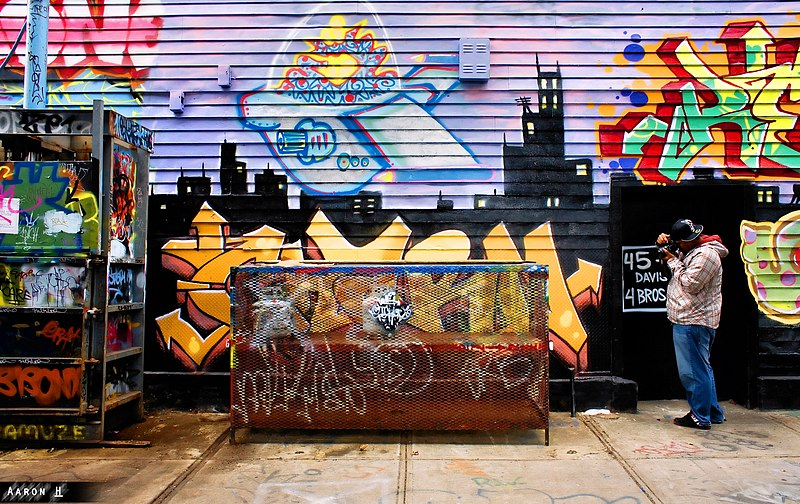
\includegraphics[width=\paperwidth]{5pointz_graffiti}}

% trick taken from https://topanswers.xyz/tex?q=1989
\tikzset{
    use page relative coordinates/.style={
        shift={(current page.south west)},
        x={(current page.south east)},
        y={(current page.north west)}
    },
}

\begin{document}
	
\begin{frame}
  \begin{tikzpicture}[remember picture, overlay,use page relative coordinates]
    
    \node[anchor=south] at (1.5-1/300*\thepage,-0.05) {
\includegraphics[width=5cm]{boom1}};
    \node[anchor=south] at (1.53-1/300*\thepage,0.01) {
\includegraphics[width=2.43cm]{th-1222073264}};    
    
    % credit for background image
    \node[white,text width=.7\paperwidth,font=\tiny,align=center] at ([yshift=0.35cm]current page.south) {Image source: \url{https://commons.wikimedia.org/wiki/File:5pointz_graffiti.jpg}};  
    
  \end{tikzpicture}
  \pause[300]
\end{frame}	
	
\end{document}